\documentclass[12pt]{article}

\usepackage[
colorlinks = true, 
linkcolor = blue, 
urlcolor = blue, 
citecolor = blue
]{hyperref}

\usepackage[romanian,english]{babel}
\usepackage{indentfirst}
\usepackage{setspace}
\usepackage{enumitem}
\usepackage{times}\usepackage{setspace} \doublespacing
\usepackage{float}
\usepackage{fontspec}
\usepackage{lilyglyphs}
\usepackage{listings}
\usepackage{minted} 
\usepackage{mdframed}
\usepackage{sourcecodepro}
\usepackage[reqno]{amsmath}
\usepackage{csquotes, multirow, graphicx, makecell}
\usepackage[a4paper, total={6in, 8in}]{geometry}

\usepackage[
backend=biber,
sorting=ynt,
]{biblatex}


\graphicspath{{./images/}}

\definecolor{bg}{rgb}{0.9,0.9,0.9}

\makeatletter
\g@addto@macro\appendix{%
  \cleardoublepage
  \hypertarget{appendixstart}{}%
  \addtocontents{toc}{
    \protect\contentsline{section}{\protect\hyperlink{appendixstart}{Anexe}}{}{}%
  }%
}
\makeatother

\newenvironment{abstractpage}
  {\cleardoublepage\vspace*{\fill}\thispagestyle{empty}}
  {\vfill\cleardoublepage}
\renewenvironment{abstract}[1]
  {\bigskip\selectlanguage{#1}%
   \begin{center}\bfseries\abstractname\end{center}}
  {\par\bigskip}
  
\newcounter{codeno}
\newcommand{\rtask}[1]{\refstepcounter{codeno}\label{#1}}
\BeforeBeginEnvironment{minted}{\addtocounter{codeno}{-1}}
\counterwithin{figure}{section}
\counterwithin{equation}{section}
\counterwithin{codeno}{section}

\addbibresource{bibliography.bib} %Imports bibliography file

\title{Generare MIDI folosind algoritmi genetici}
\author{Gheorghe Andrei}
\date{August 2022}

\makeatletter

\begin{document}

\pagestyle{empty}

\begin{titlepage}

\begin{figure}[!htb]
    \centering
    \begin{minipage}{0.2\textwidth}
        
\includegraphics[width=\linewidth]{logo-ub.png}
    \end{minipage}
    \begin{minipage}{0.5\textwidth}
        \large
        \vspace{0.2cm}
        \begin{center}
            \textbf{UNIVERSITATEA DIN BUCUREȘTI}
        \end{center}
        \vspace{0.3cm}
        \begin{center}
            \textbf{
                FACULTATEA DE \\
                MATEMATICĂ ȘI INFORMATICĂ
            }
        \end{center}
    \end{minipage}
    \begin{minipage}{0.2\textwidth}
        
\includegraphics[width=\linewidth]{logo-fmi.png}
    \end{minipage}
\end{figure}

\begin{center}
\textbf{SPECIALIZAREA INFORMATICĂ}
\end{center}

\vspace{0.5cm}

\begin{center}
\Large \textbf{Lucrare de licență}
\end{center}

\begin{center}
\huge \textbf{\@title}
\end{center}

\vspace{0.7cm}

\begin{center}
\large \textbf{Absolvent \\ \@author}
\end{center}

\vspace{0.1cm}

\begin{center}
\large \textbf{Coordonator științific \\ Lect. Dr. Sergiu Nisioi}
\end{center}

\vspace{0.3cm}

\begin{center}
\Large \textbf{București, Septembrie 2022}
\end{center}
\end{titlepage}



\selectlanguage{romanian}

\begin{abstractpage}

\begin{abstract}{romanian}
Domeniul creativității artificiale a propus sisteme de compoziție algoritmică capabile să producă rezultate impresionante. Totuși, majoritatea prezintă modele autonome, care omit interacțiunea umană din implementare. Ca rezultat, există puține unelte bazate pe compoziție algoritmică accesibile consumatorului obișnuit. Obiectivul acestei lucrări este implementerea unui sistem interactiv de unelte bazate pe algoritmi genetici și operatorii folosiți în cadrul acestora. Produsul final este împachetat sub forma unui audio plugin pentru a putea fi folosit într-un DAW și este astfel mai accesibil și ușor de folosit de către muzicieni.
\end{abstract}

\begin{abstract}{english}
The field of computational creativity has proposed algorithmic composition systems capable of producing impressive results. However, most of them are based on autonomous models, which function without ongoing human intervention. Consequently, there are few examples of algorithmic composition tools accessible to musicians. This paper proposes an interactive system driven by genetic algorithms and the genetic operators they derive. The final product is packaged as an audio plugin and can be opened by most DAWs, resulting in better accessibility and ease of use.
\end{abstract}

\end{abstractpage}

\tableofcontents

\clearpage
\addtocounter{page}{1}
\pagestyle{plain} 

\section{Introducere}
\noindent Compoziția algoritmică este o tehnică folosită frecvent de către muzicieni. Există diverse metode de a folosi compoziția algoritmică în procesul de creație muzicală: procesul poate să fie neasistat (compoziția este în total creată în mod algoritmic fără intervenția unui muzician), sau poate fi centrat în jurul componentei umane; datele generate pot acționa direct asupra undelor sonor, sau pot fi complet abstractizate de modul în care este generat suntetul, precum este generarea algoritmică de partituri muzicale. \par 
În această lucrare voi analiza compoziția algoritmică ca unealtă asistivă în procesul de creație uman și voi încerca să implementez o interfață care să permită generarea parametrizată de secvențe muzicale scurte în format MIDI. În continuarea acestui capitol voi argumenta motivul pentru care consider importantă studierea compoziției algoritmice ca procedeu stilistic și voi prezentă câteva dintre metodele actuale de implementare. 
\par Voi începe cel de-al doilea capitol prin a explica câteva noțiuni fundamentale din teoria muzicală clasică, urmând ca apoi să prezint metode matematice de modelare a noțiunilor prezentate. În continuare voi descrie câteva particularități ale formatului digital MIDI și ale extensiilor folosite în domeniul muzical digital.
\par Capitolul 3 al lucrării va conține prezentarea structurii implementării pe care o propun, precum și uneltele pe care le-am folosit pentru a configura, testa și construi aplicația.
\par Al patrulea capitol explică implementarea componentei grafice. Aici voi ilustra modul în care am utilizat componenta teoretică în cadrul implementării, precum și modul de utilizare și funcționare a plugin-ului. Cel de-al 5-lea capitol al lucrării prezintă implementarea și utilizarea algoritmilor genetici în cadrul compoziției algoritmice.
\par În final voi analiza limitările implementării prezentate, precum și modul în care aceasta poate fi îmbunătățită. Lucrarea este însoțită de două anexe, prima conține prototipurile claselor din cadrul aplicației, a doua conține fragmente de cod folosite în împlementarea componentelor și tehnologiilor diverse utilizate.
\subsection{Motivație}
\noindent Compoziția algoritmică în cadrul creației muzicale este o tehnică utilizată frecvent, care își are originile într-o oarecare formă în antichitate. Conceptul de a utiliza instrucțiuni și procese formale în cadrul compoziției muzicale își are originile în sistemul muzical utilizat în Grecia Antică \cite{website:history}, \cite{history}. Există diferite sisteme muzicale concepute în aceasta perioadă, precum sistemul de acordare Pitagorean, un algoritm care construiește o scară muzicală între două note muzicale cu rația frecvențelor 1:2. Totuși, sistemele de compoziție algoritmică nu au putut sa crească în complexitate semnificativ până la aparația sistemelor automate de calcul. Astfel, apariția calculatoarelor și a instrumentelor electronice a facilitat apariția unor noi dimensiuni muzicale, iar procesul de creație muzicală s-a schimbat fundamental. Spre exemplu, introducerea sintetizatoarelor de sunet, instrumente capabile de a genera și reda un număr nelimitat de frecvențe sonore a introdus dimensiunea complet nouă în procesul compozițional. În prezent, procesul de creație muzicală transcede regulilor uzuale definite de teoria muzicală și nu mai este în mod necesar orientat în jurul lor. Totuși, acestea încă reprezintă în general fundația peste care este construită o compoziție. Consider astfel că automatizarea acestor procese ar facilita o libertate de explorare mai mare în cadrul procesului compozițional, în special în rândul artiștilor neexperimentați.
\subsection{Implementāri existente}
\noindent Există numeroase modele folosite în implementarea sistemelor de compoziție algoritmică. Multe dintre acestea tratează problema prezenetată ca pe o problemă de optimizare, precum modelele Markov \cite{markov}, modelele bazate pe învățare ranforsată \cite{reinforced}, sau modelele evoluționare \cite{genetic_rc}, \cite{genetic_k}. Alte exemple de modele folosite sunt modelele matematice și modelele translaționale.  În implementarea propusă am ales folosirea unui model evoluționar, deoarece consider că operatorii genetici pot fi folosiți și în implementarea altor funcționalități utile în creația muzicală. Pe lânga implementările teoretice există și produse comerciale implementate: \par
\begin{itemize} 
    \item \textbf{Magenta Studio} - dezvoltat de Magenta, este o colecție de unelte muzicale implementată folosind modelele open-source de machine learning dezvoltate de companie \cite{magentastudio}. Exemple de funcționalități incluse în cadrul colecției sunt \textit{Generate}, \textit{Interpolate}, sau \textit{Drumify}. 
    \item \textbf{Bassline Studio} - \cite{website:reason} dezvoltat de Reason Studios, este un sequencer folosit pentru a genera secvențe monofonice de note \textit{reason}. Acesta este un plugin "proprietary", însă metoda prin care generează secvențe muzicale pare implementată folosind un model matematic deterministic.
\end{itemize}
    
\subsection{Contribuția personală}
    \noindent Contribuția personală adusă în cadrul acestei lucrări constă în implementarea unui plugin audio și al unui modul pe python pentru manipularea și generarea automată de fișiere MIDI. Codul sursă al plugin-ului este disponibil pe \href{https://github.com/speedypleath/b2bAI}{GitHub}. Modulul de python este publicat prin \href{https://pypi.org/project/midi-generator/}{PyPi}, iar codul sursă al acestuia este disponibil într-un alt repository de  \href{https://github.com/speedypleath/midi_generator}{GitHub}.
\section{Preliminarii}

\subsection{Elemente de teorie muzicală}
\noindent
Pentru a prezenta funcționalitățiile aplicației este necesară definirea câtorva termeni care descriu aspecte fundamentale ale melodiei. 

\subsubsection{Armonie}
\noindent Armonia reprezintă procesul prin care sunete individuale sunt aranjate în unități individuale. Fiecare notă muzicală are asociată o anumită frecvență, reprezentând numărul de oscilații produse într-o secundă de semnalul sonor obținut prin redarea sa. Raportul dintre frecvența a două note muzicale corespunde nivelului de \textit{consonanță} dintre cele două. Consonanța este atât un criteriu fizic cât și un fenomen psihologic: două note sunt considerate consonante dacaă redate împreuna formează un sunet plăcut. Astfel, o secvență muzicală este considerată \textit{armonioasă} dacă notele muzicale din care este compusă sunt consonante. \par
\noindent \textbf{Gamă} \par
\noindent Intervalul cuprins între două note cu rația frecvențelor de $2:1$ corespunde unei \textit{octave} și reprezintă baza din care se construiește fiecare \textit{gamă muzicală}. Astfel, problema construcției unei game reprezintă găsirea unei mulțimi de note consonante în acest interval \cite{history}.  În general, compozițiile muzicale sunt scrise folosind predominant note aparținând unei singure game pentru a asigura caracterul armonios. Gamele muzicale pot fi clasificate în funcție de numărul de note: 

\begin{itemize}[topsep=5pt,itemsep=2pt,parsep=0pt,partopsep=0pt]
    \item \textbf{Cromatic, sau dodecatonic} - 12 note
    \item \textbf{Nonatonic} - 9 note
    \item \textbf{Octatonic} - 8 note
    \item \textbf{Heptatonic} - 7 note
    \item \textbf{Hexatonic} - 6 note, etc.
\end{itemize} 

\begin{figure}[H]
    \centering
    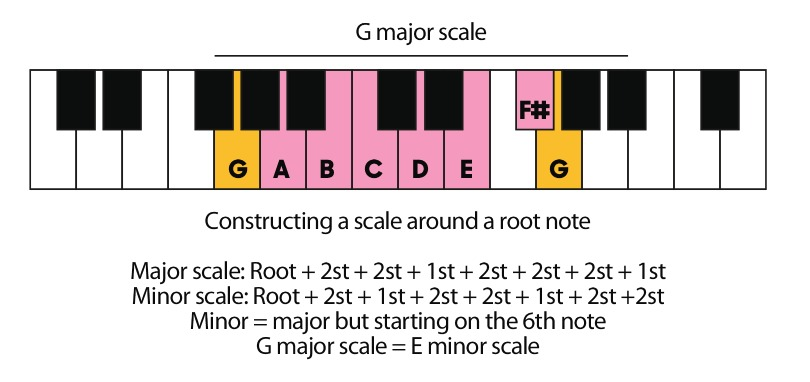
\includegraphics[scale=0.45]{images/scale.jpeg}
    \caption{Construirea unei game în jurul unei note}
    \label{image.scale}
\end{figure}

\noindent \textbf{Mod} \par
\noindent Există mai multe \textit{moduri} în care poate fi construită o gamă, în funcție distanța în frecvență dintre note. Această distanță se calculată în \textit{tonuri (t)} și \textit{semitonuri (s)}. În continuare, voi utiliza doar game heptatonice în următoarele moduri:

\begin{itemize}[topsep=0pt,itemsep=0pt,parsep=0pt,partopsep=0pt]
    \item \textbf{Aeolian (minor)}: t-s-t-t-s-t-t
    \item \textbf{Locrian}: s-t-t-s-t-t-t
    \item \textbf{Ionian: (major)} t-t-s-t-t-t-s
    \item \textbf{Dorian}: t-s-t-t-t-s-t
    \item \textbf{Phrygian}: s-t-t-t-s-t-t
    \item \textbf{Lydian}: t-t-t-s-t-t-s
    \item \textbf{Mixolydian}: t-t-s-t-t-s-t
\end{itemize}

\noindent \textbf{Acord} \par
\noindent Un acord este o combinație de note consonante redate simultan. Cele mai întâlnite acorduri sunt triadele, compuse din 3 note aparținând aceleiași game muzicale.  \par

\begin{table}[H]
    \begin{center}

    \begin{tabular}{ c c c }
        \hline
        Acord & Note & Notație \\
        \hline
        1 & G B D & I \\
        2 & A C E & ii \\
        3 & B D F\# & iii \\
        4 & C E G & IV \\
        5 & D F\# A & V \\
        6 & E G B & vi \\
        7 & F\# A C & vii \\
        \hline
    \end{tabular}
    \caption{Triadele diatonice în G major}
    \end{center}
\end{table}

\noindent O înșiruire de acorduri se numește progresie de acorduri. În general, progresiile de acorduri reprezintă fundația armoniei într-o piesă muzicală.

\subsubsection{Ritm}

\noindent Ritmul reprezintă alternarea recurentă și simetrică între elemente distincte. Ticurile unui ceas sunt un exemplu concret de ritm. Ticurile ceasului sunt evenimente despărțite în timpi egali și sunt percepute diferit (tic-tac), deși sunt identice. Gruparea impulsurilor (tic-tac) formează nivele noi de periodicitate, care compun o structura pe mai multe nivele, numită \textit{metru}. 

\begin{figure}[H]
    \centering
    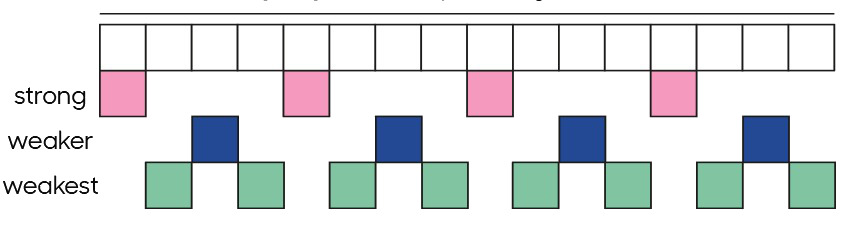
\includegraphics[scale=1.8]{images/rhythm.jpeg}
    \caption{Exemplu de metru}
    \label{image.rhythm}
\end{figure}

Alternarea periodică între \textit{impulsuri (beats) puternice} și \textit{impulsuri slabe} slabe este fundamentală pentru ideea de metru \cite{lerd}. Impulsurile puternice nu diferă într-un sens fizic (e.g. frecvență, durată, amplitudine) de cele slabe, dar sunt percepute ca fiind fundamentale. Gruparea pulsurilor in grupuri cu număr non-prim de elemente pot fi subdivizate in subgrupuri de pulsuri egale ca dimensiune. Astfel, se crează o structură metrică pe mai multe nivele \cite{sync}. În figura 2.2 sunt ilustrate nivelele metrice ale unei grupări cu 4 elemente. Pulsurile marcate cu roz se numesc \textit{downbeats}, cele marcate cu verde \textit{upbeats}, iar cele verzi \textit{backbeats}. \par
\noindent \textbf{Notă} \\
\noindent În teoria muzicală vestică, un eveniment sonor este denumit \textit{notă}, în timp ce un eveniment silențios este numit \textit{pauză}. Fiecărei note sau pauze îi este asociată o \textit{durată (sau valoare)}. Valorile notelor nu reprezintă unități absolute de timp, ci sunt definite relativ la nota întreagă. Notele pot fi acompaniate de diferite \textit{accente}, care modifică durata, frecvența(tonalitatea) sau intensitatea. \par

\begin{table}[H]
    \begin{center}
    \renewcommand{\arraystretch}{1.5}
    \begin{tabular}{ c c c c }
         \hline
         \\[-3.8em]
         Notă & Pauză & Valoarea notei & Denumire \\
         \hline
         \Large \wholeNote & \large \wholeNoteRest  & $1$ & Notă întreagă \\  
         \large \halfNote & \large \halfNoteRest & $\frac{1}{2}$ & Doime \\
         \large \crotchet & \large \crotchetRest & $\frac{1}{4}$ & Pătrime \\
         \large \quaver & \large \quaverRest & $\frac{1}{8}$ & Optime\\
         \large \semiquaver & \large \semiquaverRest & $\frac{1}{16}$ & Şaisprezecime \\
         \hline
    \end{tabular}
    \caption{Durata notelor muzicale}
    \end{center}
\end{table}

\noindent O secvență de note poate fi sincronizată cu structura metrică, caz în care aceasta devine o unitate ritmică. Există mai multe moduri prin care se poate realiza sincronizarea: \cite{rhythm}

\begin{itemize}[topsep=0pt,itemsep=0pt,parsep=0pt,partopsep=0pt]
    \item \textbf{Metric}: Valorile notelor sunt identice cu pulsurile unui nivel metric.
    \item \textbf{Intrametric}: Valorile notelor sunt bazate pe grupări de pulsuri din structura metrică dar nu sunt egale cu pulsurile din structura metrică, însă accentele lor corespund accentuării din structura metrică.
    \item \textbf{Contrametric}: Valorile notelor sunt identice cu pulsurile unui nivel metric sau sunt bazate pe grupări de pulsuri din structura metrică dar accentele lor nu corespund accentuării din structura metrică, ci o perturbă.
    \item \textbf{Extrametric}: Valorile notelor sunt bazate pe grupări de pulsuri din afara structurii metrice.
\end{itemize}

\subsubsection{Compoziție}
\noindent Structura unei secvențe muzicale diferă în funcție de instrumentul pentru care aceasta este compusă. Instrumentele muzicale pot fi \textit{monofonice} (o singură notă este redată în orice moment) sau \textit{polifonice} (mai multe note pot fi redate simultan). În funcție de rolul lor în compoziție, instrumentele pot fi încadrate în mai multe categorii, printre care: \par

\begin{itemize}
    \item \textbf{Bass:} monofonic, redă note cu frecvențe reduse (până în ~260Hz) 
    \item \textbf{Lead:} monofonic, este compus din note cu frecvențe mijlocii sau ridicate și are rolul de a reda melodia
    \item \textbf{Pad:} polifonic, este ambiental și are rolul de a stabili armonia
\end{itemize}

\subsection{Metode de măsurare a nivelului de sincopare}
\noindent Sincopa este contradicția monentană a structurii ritmice predominante i.e. o secvență de note este sincopată atunci cānd sincronizarea sa cu structura ritmică se realizează în mod contrametric \cite{rhythm}. Pentru a ilustra modul de calculare al metodelor prezentate voi folosi secvența "Bossa-Nova".

\begin{figure}[H]
    \centering
    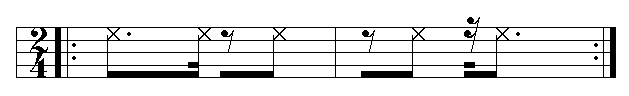
\includegraphics{images/bossa_nova.png}
    \caption{Bossa nova}
    \label{fig:bossa}
\end{figure}

\subsubsection{Gómez "Weighted Note-to-Beat"}
\label{wnbd}
\noindent Modelul "Weighted Note-to-Beat" \cite{Gomez} definește nivelul de sincopare al unei note ca fiind distanța dintre pulsurile metrului. Pentru a calcula distanța $D_{WNBD}(S)$ definim întâi $x_n$ o notă cu $x_n^s$ și $x_n^e$ începutul, respectiv sfărșitul, ${b_i}$, $b_{i+1}$ "beat-urile" între care se află, și distanța $d$.
\begin{equation}
    b_i \leq x_n^s \leq b_{i+1}
\end{equation}
\begin{equation}
    d(x_n, b_i) = \frac{x_n^s - b_i}{b_{i+1}-b_i}
\end{equation}
În continuare definim $T(x_n)$ ca fiind distanța dintre ${x_n}$ și cel mai apropiat beat.
\begin{equation}
    T(x_n) = min(d(x_n, b_i), d(x_n, b_{i+1}))
\end{equation}
Valoarea $W(x_n)$ reprezintă nivelul de sincopare al unei note și se calculează astfel:
\begin{equation}
    W(x_n) = 
    \begin{cases}
        \hfil 0, & \text{dacă } d(x_n, b_i) = 0 \\
        \frac{2}{T(x_n)}, & \text{dacă } b_{i+1} < x_n^e \leq b_{i+2} \\
        \frac{1}{T(x_n)}, & \text{altfel}
    \end{cases}
\end{equation}
În final, nivelul de sincopare al unei structuri ritmice se calculează astfel:
\begin{equation}
    D_{WNBD}(S) = \frac{1}{|Y|}\sum_{n=0}^{|Y|-1}{W(x_n)}
\end{equation}

Spre exemplu, pentru secvența Bossa-Nova ponderile notelor sunt (0, 4, 8, 8, 4), deci WNBD prezice un nivel de sincopare de valoare 3.

\subsubsection{Toussaint "Off-Beatness"}
\label{ob}
\noindent Modelul "Off-Beatness" \cite{Toussaint} definește o notă ca fiind sincopată atunci câ este redată în timpul unui puls "off-beat". Un puls este considerat off-beat dacă începe în același timp cu un puls din mulțimea formată din generatorii grupului ciclic $C_{n}$, unde $n$ este numărul de pulsuri al metrului. Pentru a calcula nivelul de sincopare $D_{TOB}$ al unei structuri ritmice definim întâi $B$ ca fiind mulțimea numerelor non-prime față de $n$ .
\begin{equation}
    B = \{i, \: n \text{ mod } i = 0 : 1 < i < n\}
\end{equation}
Valoarea $W(x_n)$ reprezintă nivelul de sincopare al unei note și se calculează astfel:
\begin{equation}
    W(x_n) = 
    \begin{cases}
        0, & \text{dacă $x$ mod } i = 0 \: \forall \: i \in B\\
        1, & \text{altfel}
    \end{cases}
\end{equation}
În final, nivelul de sincopare al unei structuri ritmice se calculează folosind modelul "Off-Beatness" astfel:
\begin{equation}
    D_{TOB}(S) = \frac{1}{|Y|}\sum_{n=0}^{|Y|-1}{W(x_n)}
\end{equation}
Pentru secvența Bossa-Nova conține 16 pulsuri, iar notele sunt distribuite astfel: [x..x..x...x..x..]. Așadar, a 2-a și a 5-a sunt offbeat, deci nivelul de sincopare prezis este 2.

\subsection{Formatul MIDI}
\noindent Formatul MIDI (Musical Instrument Digital Interface) este un standard tehnic care descrie un protocol de comunicații, o interfață digitală și tipuri de conectori electrici care conectează instrumente muzicale electronice și dispozitive audio. Informația MIDI este transmisă prin \textit{mesaje MIDI}. Acestea sunt formate dintr-un \textit{status byte}, urmat de unul sau mai mulți \textit{data bytes} și pot fi clasificate drept "System Messages, "Channel Voice Messages" și "channel mode messages". \cite{midi} \par
\noindent \textbf{Channel Voice Messages} \par 
\noindent Channel Voice Messages sunt folosite pentru a transmite informații legate de performanța muzicală și sunt de tipul \textit{Note On, Note Off, Polyphonic Key Pressure, Channel Pressure, Pitch Bend Change, Program Change}, sau \textit{Control Change messages}. O notă muzicală este transmisă pentru a fi redată folosind un mesaj de tipul Note On, indicāndu-se nota (tonică) și velocitatea, urmat de un mesaj de tipul Note Off. Astfel, durata notei este calculată în funcție de diferența dintre timpii la care s-au primit cele 2 evenimente. \par
\noindent \textbf{Channel Mode Messages} \par
\noindent Channel Mode Messages afectează modul în care sintetizatoarele răspund datelor MIDI. Acestea pot fi folosite pentru Acestea pot fi folosite pentru a selecte între a reda note monofonic sau polifonic.\par
\noindent \textbf{System Messages} \par
\noindent System Messages diferă de celelalte două tipuri prin faptul că nu sunt specifice unui singur canal, deci nu includ un număr de canal în status byte. Acestea pot fi folosite pentru a sincroniza instrumente, sau pentru a transmite mesaje definite exclusiv pentru anumite echipamente.
\noindent \par

\subsection{Audio plugin}

\noindent Un plugin audio este un plugin folosit pentru a adăuga sau îmbunătății funcționalități audio într-un program, în general un DAW (Digital Audio Workstation). Există mai multe arhitecturi care funcționează diferit în funcție de sistemul de operare sau DAW, cele mai utilizate fiind: \par
\begin{itemize}
    \item \textbf{VST (Virtual Studio Technology):} cel mai utilizat format, cross-platform
    
    \item \textbf{AU (AudioUnits):} creat de Apple special pentru MacOS
\end{itemize}
\noindent \textbf{JUCE} \par
\noindent JUCE este un framework de C++ cross-platform folosit pentru a crea audio plugins. Acesta implementează multiple funcționalități audio și oferă posibilitatea exportării proiectelor în majoritatea formatelor.
\section{Arhitectura aplicației} \label{arhitectura}
    \noindent Aplicația conține un audio plugin exportat în format VST3, AU și Standalone scrisă în C++ folosind JUCE, un modul scris în python pentru generarea secvențelor muzicale, precum și o librărie comună scrisă în C++ folosind Pybind11. 
    \begin{figure}[H]
        \centering
        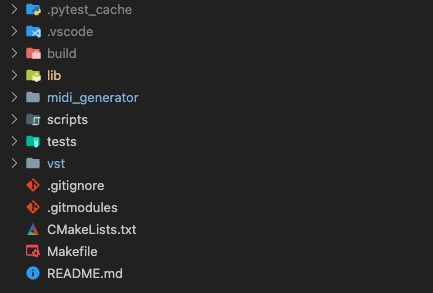
\includegraphics[scale=0.6]{images/structura.jpeg}
        \caption{Structura proiectului după build}
        \label{fig:structure}
    \end{figure}
    
    \subsection{Structură}
        \noindent Aplicația e construită folosind cmake și make, și a fost testată pe Debian 11 ARM și macOS 12. Pentru a putea utiliza aplicația, următoarele dependențe trebuiesc instalate:
        \begin{itemize}
            \item Python 3.10 (versiunea dev)
            \item CMake 3.23
            \item Make 4.3
            \item Clang 11
        \end{itemize}
        
    \subsection{Librării}
        \noindent \textbf{Boost} \par
        \noindent Boost este o colecție de librării scrise în C++ care implementează funcționalități folosite frecvent în dezvoltarea software. Dintre acestea, am folosit librăriile de logging și cel de testare unitară. \par 
        \noindent \textbf{Pybind11} \par
        \noindent Pybind11 este o librărie care permite interoperabilitate între C++ și python. Aceasta este folosită în aplicație pentru a facilita crearea unei interfețe de comunicare între plugin și modulul genetic. Un exemplu conținând implementarea endpoint-ului pentru apelarea funcției de generare din cadrul algoritmului genetic se poate găsi în Anexa \ref{Boost}. \par
    
    \subsection{Build tools}
        \noindent \textbf{Make} \par
            \noindent Pentru construirea, testarea și depanarea aplicației am folosit Make și CMake. În Make sunt definite 7 sarcini executabile:
            \begin{itemize}
                \item \textbf{config} - configurează structura proiectelor CMake.
                \item \textbf{build-lib} - construiește librăria comună folosită de plugin si modul.
                \item \textbf{build} - construiește modulul de python și pluginul standalone.
                \item \textbf{test} - execută testele unitare conținute în aplicație.
                \item \textbf{run} - rulează pluginul standalone.
                \item \textbf{clean} - șterge folder-ul în care este construită aplicația (build) și fișierele temporare create de python.
                \item \textbf{all} - execută în ordinea config\rightarrow build-plugin\rightarrow build\rightarrow test\rightarrow run.
            \end{itemize}
        \noindent \textbf{Cmake} \par
            \noindent CMake este unealta de împachetare principală folosită. Aplicația folosește 4 fișiere de configurare pentru crearea executabilului final. Primul dintre acestea este conținute în directorul principal al aplicației și reprezintă punctul de început al configurație (Anexa \ref{CMake}). Aici sunt căutate librăriile din python și boost și executabilul de python și sunt incluse în configurație, după care este configurată librăria comună și este construit și instalat modulul genetic. Apoi, sunt adăugate și configurate modulele folosite în cadrul plugin-ului, urmate de plugin-ul audio și configurarea testelor. \par
            Următorul fișier de configurare este localizat în directorul în care este conținută librăria comună și are scopul de a o construi și adăuga în configurație. Directorul în care se crează plugin-ul audio conține de asemenea un fișier de configurare, care crează executabilele în format .VST, .AU și Stanadalone, și include modulele folosite. Ultimul fișier este localizat în directorul care conține testele unitare și este folosit pentru a crea mai multe executabile, reprezentând suite de teste.
        
    \subsection{Testare}
        \noindent Aplicația conține teste unitare scrise folosind pytest (pentru testarea modulului) și librăria de teste unitare conținute în boost (pentru librărie comună și plugin-ul audio). Acestea sunt folosite în special pentru a verifica daca este configurată corect comunicarea între componentele distincte ale aplicației. 
        \par Un exemplu de suită de teste este inclusă în anexa \ref{Testare}, folosit pentru a verifica dacă librăria poate traduce informație legată de notele muzicale din Python în C++ și invers. Celelalte suite de teste verifică dacă librăria dinamică este încarcată corect la runtime, funcționarea corespunzătoare a API-ului și funcționarea comenzilor conținute în modulul genetic.
 
\section{Implementarea plugin-ului audio} 
    \label{plugin}
    \noindent Plugin-ul audio este implementat în C++ folosind framework-ul JUCE, împreună cu modulul PluginGuiMagic  \cite{website:1}. Clasa MagicProcessor din modulul PluginGuiMagic extinde clasa AudioProcessor și reprezintă clasa de bază din care este derivat punctul de început al plugin-ului.
    \begin{figure}[H]
        \centering
        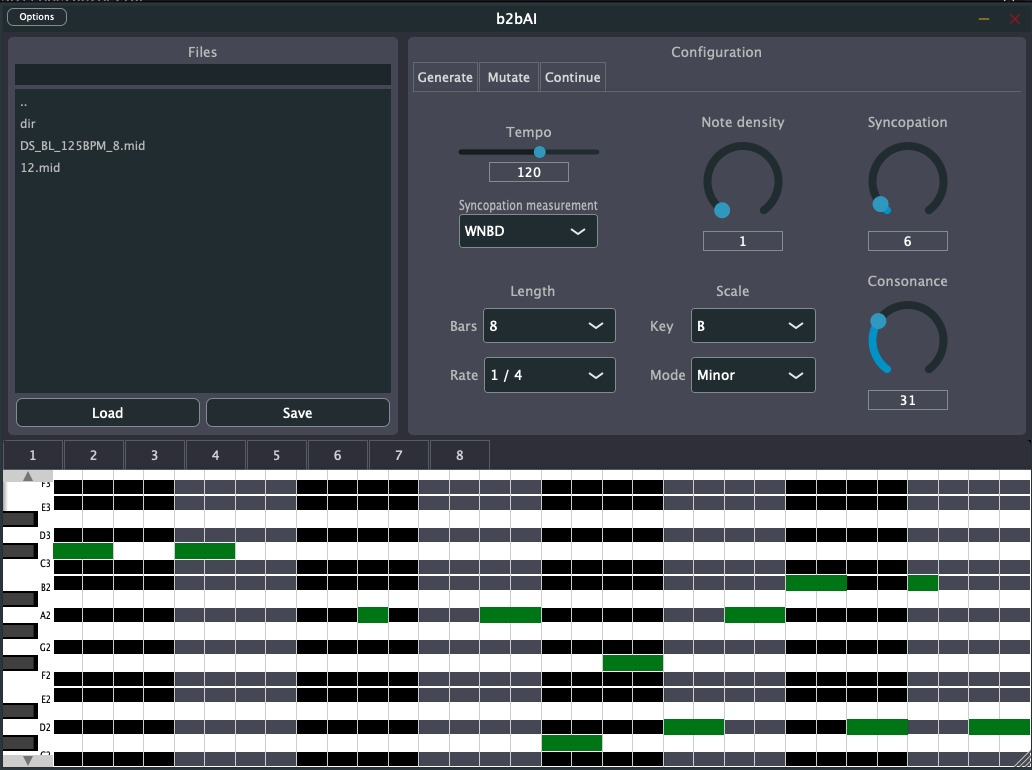
\includegraphics[scale=0.3]{images/interfata.jpeg}
        \caption{Interfața grafică a plugin-ului}
        \label{fig:interfata}
    \end{figure}
    \subsection{B2bAIPluginProcessor}
    \noindent Interfața grafică a plugin-ului este creată dintr-un fișier XML, care conține o structură arborescentă de componente (Anexa \ref{XML}). Acesta este încarcat în constructor-ul clasei B2bAIPluginProcessor (Anexa \ref{B2bAIAudioProcessor}), care extinde clasa MagicProcessor și reprezintă componenta principală a plugin-ului. Clasa crează de asemenea parametrii audio și celelalte resurse dinamice și le atașează componentelor corespunzătoare. În plus, aceasta recepționează și procesează mesaje MIDI și evenimente audio. \par
    Metoda initialiseBuilder, care suprascrie metoda virtuală a clasei MagicProcessor, permite înregistrarea de componente noi refolosibile.
    \begin{minted}[fontsize=\footnotesize, baselinestretch=1]{c++}
void B2bAIAudioProcessor::initialiseBuilder 
                            (foleys::MagicGUIBuilder& builder)
{
    builder.registerJUCEFactories();

    builder.registerFactory ("PianoRoll", &PianoRoll::factory);
    builder.registerFactory ("SearchBar", &SearchBar::factory);
}
    
    \end{minted}
    \subsection{Piano roll}
        \noindent Piano roll-ul permite vizualizarea și editarea notelor dintr-o secvență. Opt secvențe pot fi editate simultan; pentru a încarcă o secventă în piano roll se folosesc tab-urile numerotate de la 1 la 8. Notele pot fi adaugate, șterse,  mutate sau redimensionate pe grid folosind mouse-ul, valorile notelor (tonice) pot fi derulate folosind mousewheel-ul. \par
        Piano roll-ul este implementat folosind clasa PianoRollComponent (Anexa \ref{PianoRollComponent}), care încapsulează 2 componente: un pian (KeyboardComponent) și un un grid (GridComponent). Pianul este un reskin al componentei JUCE::MidiKeyboardComponent. Grid-ul este o matrice construită dinamic în funcție de evenimentele generate de mouse, numărul de pulsuri al metrului și o listă de note inițializată la runtime (Anexa \ref{Update}). \par 
                \begin{figure}[H]
            \centering
            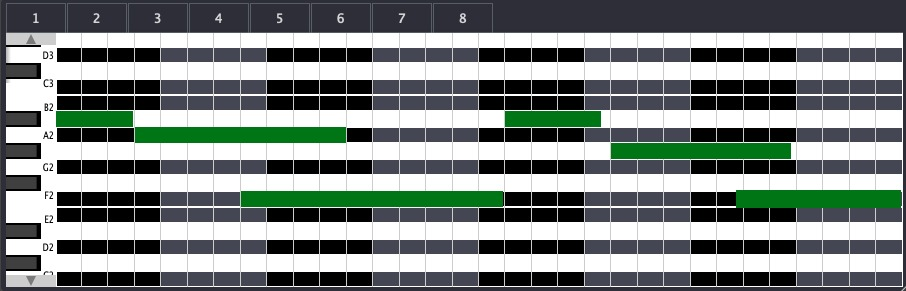
\includegraphics[scale=0.428]{images/pianoroll.jpeg}
            \caption{Piano roll}
            \label{fig:piano_rol}
        \end{figure}
        \noindent Wrapper-ul PianoRoll (Anexa \ref{PianoRoll}) încapsulează această clasă PianoRollComponent și este folosit pentru a o înregistra drept componentă reutilizabilă în B2bAIAudioProcessor::initialiseBuilder. În plus, wrapperul prezintă și o interfață pentru a inițializa și actualiza referința către lista de note din grid. \par
        
        \begin{figure}[H]
            \centering
            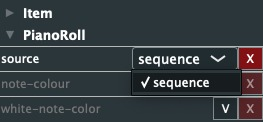
\includegraphics[scale=0.6]{images/interface.jpeg}
            \caption{Selectarea secvenței din piano roll}
            \label{fig:interface}
        \end{figure}
        
    \subsection{Sistemul de fișiere}
        \noindent Sistemul fișier de interne poate fi navigat din aplicației. Secvența MIDI asociată piano roll-ului poate fi salvată ca fișier intern. De asemenea un fișier în format MIDI poate fi descărcat și editat în piano roll.
        \begin{figure}[H]
            \centering
            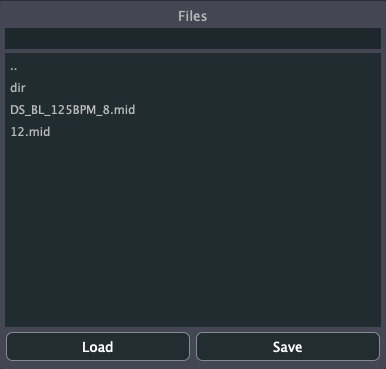
\includegraphics[scale=0.5]{images/files.jpeg}
            \caption{File tree}
            \label{fig:files}
        \end{figure}
        \noindent Implementarea este realizată folosind clasa MidiFileListBox (Anexa \ref{MidiFileListBox}), care extinde clasele ListBoxModel, ChangeBroadcaster, ChangeListener și Label::Listener. Astfel, aceasta definește 3 funcții care sunt implementate în procesorul audio, care modifică setările comune ale aplicației, și actualizează starea componentelor interioare de fiecare dată când sunt apelate. În plus, acest lucru se întâmplă și pentru chenarul de deasupra, actualizarea având loc în momentul în care este schimbată valoarea din chenar. Chenarul este definit în clasa SearchBar (Anexa \ref{SearchBar}) și este înregistrat drept componentă reutilizabilă.
    \subsection{Parametrii audio}
        \noindent Parametrii audio ai aplicației sunt folosiți pentru a configura algoritmul genetic. Fiecare dintre cele 4 funcționalități ale aplicației are parametrii de configurație proprii. \par
        \noindent \textbf{Generate}
        \begin{itemize}
            \item Syncopation - nivelul de sincopare
            \item Note density - densitatea notelor
            \item Consonance - proporția notelor consonante
            \item Key - gama în care este generată secvența
            \item Mode - modul gamei
            \item Tempo - tempo-ul secvenței; este folosit în scrierea fișierelor midi
            \item Bars - numărul de măsuri al secvenței
            \item Rate - durata unui puls
            \item Syncopation measurement - algoritmul folosit pentru măsurarea sincopării 
        \end{itemize}
        \noindent \textbf{Mutate}
        \begin{itemize}
            \item Pitch - rata de mutație a frecvenței
            \item Velocity - rata de mutație a velocității
            \item Duration - rata de mutație a lungimilor notelor
            \item Consonance - proporția notelor consonante
        \end{itemize}
        \noindent \textbf{Continue}
        \begin{itemize}
            \item Compression method: algoritmul folosit pentru compresia secvențelor
        \end{itemize}
        \noindent \textbf{Combine}
        \begin{itemize}
            \item Compression method: algoritmul folosit pentru compresia secvențelor
            \item Sequences: secvențele folosite în combinare
        \end{itemize}
       
\section{Modulul midi-generator}
    \noindent Modulul \textit{midi\hyphen generator} este un modul scris în Python care folosește librăria deap \cite{deap} pentru a implementa diverse funcționalități folosind algoritmi genetici. Acesta conține atât o interfață de linie de comandă pentru a putea fi folosit de sine stătător, cât și un API care prezintă funcționalitățiile implementate. Modulul este construit, testat și distribuit automat prin github actions la fiecare acțiune de push sau merge pe branch-ul principal de GitHub.
        
    \subsection{Algoritmul genetic}
        \noindent Algoritmul genetic este implementat folosind deap, un framework care oferă o colecție de unelte compusă din modulul \textit{creator} și modulul \textit{toolbox}. Primul modul permite creerea de clase noi care pot fi folosite în cadrul genotipului, iar al doilea reprezintă un container pentru operatorii genetici. \par
        \subsubsection{Codificare}
            \noindent Pentru a rezolva problema codificării unei secvențe de note muzicale am definit întâi clasa Gene:

            \begin{minted}[fontsize=\footnotesize, baselinestretch=1]{python}
@dataclass
class Gene:
    pitch: int
    velocity: int
    remaining_ticks: int
            \end{minted}

            \noindent Astfel, genele sunt reprezentate de pulsurile metrului folosit și conțin frecvența, velocitatea și numărul de pulsuri rămase din nota redată la momentul respectiv. Pentru a putea înregistrata genotipul în toolbox am creat un generator (Anexa \ref{generator}) de note continue în timp, de lungime variată. Acesta este implementat folosind un closure care reține valoarea notei anterioare. Funcția de generare din cadrul closure-ului verifică dacă pulsul curent are loc în timpul redării notei anterioare, caz în care returnează nota precedentă, din care este scăzut un tick. În caz contrar, generatorul returnează o notă aleatoare. Așadar, un individ reprezintă o listă formată din rezultatele returnate de generator. Înregistrarea notei în toolbox se realizează în felul următor:
            
            \begin{minted}[fontsize=\footnotesize, baselinestretch=1]{python}
creator.create("Individual", list, fitness=creator.Fitness)
toolbox.register("individual", tools.initRepeat, 
    -> creator.Individual, toolbox.generator, n=NO_TICKS)
toolbox.register("population", tools.initRepeat, list, 
    -> toolbox.generator)
            \end{minted}
            
        \subsubsection{Mutație} \par
            \noindent Mutația (Anexa \ref{mutație}) poate afecta frecvența, velocitatea sau durata unei note. În cazul în care mutația modifică durata unei note, aceasta poate afecta mai multe gene simultan (valabil și în cadrul crossover-ului). Pentru a rezolva această problemă am definit un decorator (Anexa \ref{wrapper}) care parcurge pulsurile cromozomului rezultat în urma mutației (sau a crossover-ului) și setează valoarea numărului de pulsuri rămase din notă ca fiind egală cu numărul de gene imediat consecutive care au valoare frecvenței egală cu cea a pulsului curent. Modul prin care sunt decorate cele 2 funcții este următorul: 
            
                    \begin{minted}[fontsize=\footnotesize, baselinestretch=1]{python}
decorator = check_remaining_ticks()
toolbox.decorate("mate", decorator)
toolbox.decorate("mutate", decorator)
                    \end{minted}
                    
        \subsubsection{Fitness} \par
            \noindent Funcția de fitness este calculată în funcție de nivelul de sincopare, densitatea notelor și rația notelor consonante. Pentru calcularea nivelului de sincopare, se poate alege între măsura WNBD (Capitolul \ref{wnbd}, implementare Anexa \ref{WNBD}) și off-beatness (Capitolul \ref{ob}, implementare Anexa \ref{offbeatness}). Densitatea și rația notelor consonante sunt calculate prin raportul dintre numărul de pulsuri în care sunt redate note, respectiv numărul de pulsuri în care sunt redata note din gama selectată și numărul total de pulsuri. \par
            Pentru funcțiile continue și combine funcția de fitness este calculată folosind distanța NCD (Normalized
Compression Distance) care se calculează prin formula:
            \begin{equation}
                NCD(x, y) = \frac{ max(C(xy) - C(x), C(yx) - C(y)) }{ max( C(x), C(y) ) }
            \end{equation}
            \noindent Unde $C(x)$ reprezintă lungimea rezultatului compresiei lui $x$ folosind orice algoritm aproximativ pentru complexitatea Kolmogorov \cite{kolmogovorv}. Astfel, pentru un set de secvențe $S$ și un individ $x$ funcția de fitness este dată de formula: 
            \begin{equation}
                f(x) = \frac{1}{ \sum\limits_{s \in S}{NCD(x, s)} }
            \end{equation}
            \noindent În aplicație sunt implementați 3 algoritmi de compresie, anume LZ77 \cite{lz77}, LZ78 \cite{lz78} și LZW \cite{lzw}. Implementarea algoritmului LZ77 se poate găsi în Anexa \ref{lz77}.
    \subsection{API}
        \noindent Modulul expune funcționalitățiile implementate sub forma unui API format din următoarele endpoints: \par
            \begin{itemize}
                \item \textbf{mutate} - primește ca argument o configurație; returnează o secvență de note generate folosind algoritmul genetic, în funcție de configurația primită 
                \item \textbf{continue} - primește ca argumente o secvență de note și o configurație; returnează rezultatul aplicării operatorului de mutație pe secvența de note, în funcție de configurația primită
                \item \textbf{continue} - primește ca argumente o secvență de note și o configurație; returnează o secvență de note generate folosind algoritmul genetic cu funcția de fitness kolmogorov, în funcție de configurația și secvențele primite
                \item \textbf{combine} - primește ca argumente o listă de secvențe de note și o configurație; returnează o secvență de note generate folosind algoritmul genetic cu funcția de fitness kolmogorov, în funcție de configurația și secvențele primite
                \item \textbf{write\_file} - primește ca argumente o secvență de note și calea unui fișier; scrie în calea primită un fișier MIDI format din secvența de note transmisă ca argument
            \end{itemize}
\section{Concluzii}
\noindent În această lucrare am implementat o colecție de unelte care poate asista muzicienii în procesul de creație, incluzând unelte pentru generarea, mutația, continuarea și combinarea de secvențe muzicale. Acestea sunt configurabile, păstrând astfel expresia creativă a utilizatorului. 
\subsection{Limitări ale aplicației}
\noindent Deși aplicația reprezintă un plugin audio, aceasta nu interacționează deloc cu DAW-ul din care este deschisă; pentru a putea folosi aplicația în cadrul unui DAW este nevoie ca secvențele generate să fie salvate în format MIDI, după care să fie deschise în DAW. \par
În cadrul evaluării fitness-ului unei secvențe velocitatea notelor nu este deloc utilizată, astfel că o dimensiune muzicală care ar putea fi fost folosită în cadrul generării nu este deloc valorificată. În plus, momentan aplicația nu poate genera secvențe polifonice, fiind limitată astfel mulțimea de tipuri de instrumente pentru care pot fi generate secvențe. \par
\subsection{Posibile dezvoltări ulterioare}
\noindent Plugin-ul ar putea interacționa cu DAW-ul în care este deschis folosind mesaje trimise pe MIDI Chanels. Acestea ar putea fi folosite pentru a reda sau a înregistra secvența într-un track. De asemenea, designul interfeței grafice ar putea fi îmbunătățit. \par
Velocitatea ar putea fi folosită pentru a accentua sau diminua momentele de tensiune create de notele consonante sau pentru a schimba nivelul de sincopare al unei secvențe. Secvențele polifonice ar putea fi generate folosind acorduri și progresii de acorduri. Pentru a identifica si valorifica expresiile muzicale dintr-o secvență, generarea ar putea fi implementată folosind optimizare swarm în loc de algoritmi genetici, utilitățiile necesare fiind prezente în modulul deap.


\printbibliography

\appendix
\section{Header files}

\begin{minted}[fontsize=\footnotesize, linenos=true, bgcolor=bg, frame=lines, label=PluginProcessor.h, breaklines=true, escapeinside=@@, baselinestretch=1]{c++}
@\rtask{B2bAIAudioProcessor}@
{
public:
    B2bAIAudioProcessor();
    ~B2bAIAudioProcessor() override;

    void prepareToPlay (double sampleRate, int samplesPerBlock) override;
    void releaseResources() override;

#ifndef JucePlugin_PreferredChannelConfigurations
    bool isBusesLayoutSupported (const 
            AudioProcessor::BusesLayout& layouts) 
            const override;
#endif
    void processBlock (AudioBuffer<float>&, MidiBuffer&) override;
    void saveMidiFile();
    void loadMidiFile(const File& file);
    void loadDirectory(const File& file);
    void updateListBox(const String& text);
    double getTailLengthSeconds() const override;

private:
    MidiFileListBox *midiFileListBox;
    MidiSequence *midiSequence;
    File midiFilesDir;
    AudioProcessorValueTreeState treeState;
    JUCE_DECLARE_NON_COPYABLE_WITH_LEAK_DETECTOR (B2bAIAudioProcessor)
    File getFile(int index);
    void initialiseBuilder(foleys::MagicGUIBuilder &builder) override;
};
\end{minted}

\begin{minted}[fontsize=\footnotesize, linenos=true, bgcolor=bg, frame=lines, label=PianoRollComponent.h, breaklines=true, escapeinside=@@, baselinestretch=1]{c++}
@\rtask{PianoRollComponent}@
class PianoRollComponent: public Component {
private:
    std::unique_ptr<KeyboardComponent> keyboardComponent;
    std::unique_ptr<GridComponent> gridComponent;
    void timerCallback() override;
public:
    enum ColourIds {
        noteColour = 0x00FF00
    };

    PianoRollComponent(MidiKeyboardState& state, 
            KeyboardComponent::Orientation orientation);
    void paint (juce::Graphics&) override;
    void resized() override;
    void mouseWheelMove(const MouseEvent &event, 
    const MouseWheelDetails &wheel) override;
    void setMidiSequence(MidiSequence *sequence);
};

\end{minted}

\begin{minted}[fontsize=\footnotesize, linenos=true, bgcolor=bg, frame=lines, label=MidiFileListBox.h, breaklines=true, escapeinside=@@, baselinestretch=1]{c++}
@\rtask{MidiFileListBox}@
class MidiFileListBox: public ListBoxModel,
                       public Label::Listener,
                       public ChangeBroadcaster,
                       public ChangeListener {
private:
    File midiFilesDir;
    Array<File> midiFiles;
    foleys::SharedApplicationSettings settings;
    String searchText;

    JUCE_DECLARE_NON_COPYABLE_WITH_LEAK_DETECTOR (MidiFileListBox)
public:
    MidiFileListBox();
    ~MidiFileListBox() override;

    void listBoxItemClicked (int rowNumber, const juce::MouseEvent& event) override;
    void listBoxItemDoubleClicked(int row, const juce::MouseEvent &) override;
    void paintListBoxItem (int rowNumber, juce::Graphics &g, int width, int height, bool rowIsSelected) override;

    void labelTextChanged(juce::Label *labelThatHasChanged) override;
    int getNumRows() override;
    void changeListenerCallback (juce::ChangeBroadcaster*) override;
    std::function<void(File file)> onSelectionChanged;
    std::function<void(File file)> onDoubleClick;
    std::function<void(String text)> update;
};

\end{minted}


\begin{minted}[fontsize=\footnotesize, linenos=true, bgcolor=bg, frame=lines, label=SearchBar.h, breaklines=true, escapeinside=@@, baselinestretch=1]{c++}
@\rtask{SearchBar}@
class SearchBar : public foleys::GuiItem
{
private:
    juce::Label label;
    Label::Listener *listener = nullptr;

    JUCE_DECLARE_NON_COPYABLE_WITH_LEAK_DETECTOR (SearchBar)
public:
    FOLEYS_DECLARE_GUI_FACTORY (SearchBar)

    static const juce::Identifier  pText;
    static const juce::Identifier  pJustification;
    static const juce::Identifier  pFontSize;
    static const juce::Identifier  pDestination;

    SearchBar (foleys::MagicGUIBuilder& builder, const juce::ValueTree& node);
    void update() override;
    std::vector<foleys::SettableProperty> getSettableProperties() const override;
    juce::Component* getWrappedComponent() override;
};
\end{minted}

\begin{minted}[fontsize=\footnotesize, linenos=true, bgcolor=bg, frame=lines, label=NoteRectangle.h, breaklines=true, escapeinside=@@, baselinestretch=1]{c++}
@\rtask{NoteRectangle}@
class NoteRectangle: public Rectangle<int> {
public:
    NoteRectangle(int x=0, int y=0, int width=0, int height=0, int p=0);
    NoteRectangle(int p, int v, double s, double e);
    [[nodiscard]] int getPitch() const;
    void setPitch(int pitch);
    friend std::ostream &operator<<(std::ostream &os, const NoteRectangle &note);
    [[nodiscard]] int getVelocity() const;
    void setVelocity(int velocity);
    bool operator==(const NoteRectangle &rhs) const;
    bool operator!=(const NoteRectangle &rhs) const;
    [[nodiscard]] double getStart() const;
    void setStart(double start);
    [[nodiscard]] double getEnd() const;
    void setEnd(double end);
private:
    Note note;
};
\end{minted}

\begin{minted}[fontsize=\footnotesize, linenos=true, bgcolor=bg, frame=lines, label=GridComponent.h, escapeinside=@@, breaklines=true, baselinestretch=1]{c++}
@\rtask{GridComponent}@
class GridComponent: public Component {
private:
    OwnedArray<Range<int>> noteLineRanges;
    OwnedArray<Range<int>> noteRowRanges;
    MidiSequence *notes = nullptr;
    NoteRectangle pressed, new_position;
    NoteRectangle find_note_rect(Point<int> position);
    int normalise(double w, double wMax);
public:
    GridComponent();

    void updateNoteLineRanges(int firstKeyStartPosition);

    void paint(Graphics &g) override;
    void mouseMove(const MouseEvent &event) override;
    void mouseDown(const MouseEvent &event) override;
    void mouseDrag(const MouseEvent &event) override;
    void mouseDoubleClick(const MouseEvent &event) override;
    void mouseUp(const MouseEvent &event) override;
    void setMidiSequence(MidiSequence *sequence);
};
\end{minted}

\begin{minted}[fontsize=\footnotesize, linenos=true, bgcolor=bg, frame=lines, label=PianoRoll.h, escapeinside=@@, breaklines=true, baselinestretch=1]{c++}
@\rtask{PianoRoll}@
class PianoRoll: public foleys::GuiItem {
private:
    PianoRollComponent pianoRoll;

    JUCE_DECLARE_NON_COPYABLE_WITH_LEAK_DETECTOR(PianoRoll)
public:
    FOLEYS_DECLARE_GUI_FACTORY(PianoRoll)

    static const juce::Identifier  pSource;
    static const juce::Identifier  pNoteColor;

    PianoRoll(foleys::MagicGUIBuilder& builder, const juce::ValueTree& node);

    void update() override;

    [[nodiscard]] std::vector<foleys::SettableProperty> getSettableProperties() const override;

    juce::Component* getWrappedComponent() override;
};
\end{minted}

\newpage

\section{Referințe cod} 
\begin{minted}[fontsize=\footnotesize, linenos=true, bgcolor=bg, frame=lines, label=Arbore XML, escapeinside=@@, breaklines=true, baselinestretch=1]{xml}
@\rtask{XML}@
<View background-color="FF4E505F" height="10%" display="flexbox" margin="0"
      padding="0" flex-align-self="stretch" flex-direction="column"
      radius="0" border="0" caption="Search" caption-size="0">
  <SearchBar font-size="16.0" justification="top-left" label-background="212c31"
             text="" max-height="25" height="" flex-align-self="stretch" margin="0"
             padding="1" border="0" label-outline="FF4E505F" background-color="FF4E505F"
             radius="0" caption="SearchBox" caption-size="0" pos-x="0%" pos-y="0%"
             pos-width="100%" pos-height="8.25083%" destination="filetree"/>
  <ListBox list-box-model="filetree" pos-x="0" background-color="FF4E505F"
           pos-y="0%" pos-width="100%" pos-height="10.7527%" padding="2"
           caption="FileTree" caption-size="0"/>
</View>
\end{minted}

\begin{minted}[fontsize=\footnotesize, linenos=true, bgcolor=bg, frame=lines, label=Paint grid, escapeinside=@@, breaklines=true, baselinestretch=1]{c++}
@\rtask{Update}@
void GridComponent::paint(Graphics& g)
{
    int height = getHeight();
    int width = getWidth();
    // Draw the background
    for (int i = 0; i < 8; i += 2) {
        auto shadow = DropShadow(Colours::black, 1, Point<int>(0, 0));
        auto rect = Rectangle<int>(noteRowRanges[i * 4]->getStart(),
                                   0,
                                   noteRowRanges[(i + 1) * 4]->getStart() - noteRowRanges[i * 4]->getStart(),
                                   height);
        shadow.drawForRectangle(g, rect);
    }
    g.setColour(Colours::white);

    // Draw note lines
    for (int i = 0; i < noteLineRanges.size(); i++) {
        auto rect = Rectangle<int>(0, noteLineRanges[i]->getStart(), width, noteLineRanges[i]->getLength());
        if (rect.getBottom() < 0 || rect.getY() >= height)
            continue;
        g.drawRect(rect, 1);
        if (!MidiMessage::isMidiNoteBlack(i))
            continue;
        g.fillRect(rect);
    }

    g.setColour(Colours::lightgrey);
    // Draw beats lines
    for (auto noteRowRange : noteRowRanges) {
        g.fillRect(static_cast<int>(noteRowRange->getStart() - 1), 0, 1, height);
    }

    // draw notes
    g.setColour(Colours::green);
    if(notes)
        for (const auto& note : *notes) {
            if(pressed == note) {
                g.fillRect(new_position.expanded(1));
                continue;
            }

            g.fillRect(note);
        }
}
\end{minted}

\begin{minted}[fontsize=\footnotesize, linenos=true, bgcolor=bg, frame=lines, label=Pybind11, escapeinside=@@, breaklines=true, baselinestretch=1]{c++}
@\rtask{Boost}@
std::list<mg::Note> mg::generate() {
    try {
        pybind11::module_ commands = pybind11::module_::import("midi_generator.commands");
        py::object result = commands.attr("generate")();
        std::list<mg::Note> notes;
        for(const auto& obj: result)
            notes.emplace_back(
                    obj.attr("pitch").cast<int>(),
                    obj.attr("velocity").cast<int>(),
                    obj.attr("start").cast<double>(),
                    obj.attr("end").cast<double>()
                    );

        return notes;
    } catch (py::error_already_set &error) {
        error.discard_as_unraisable(__func__ );
        return {};
    }
}
\end{minted}

\begin{minted}[fontsize=\footnotesize, linenos=true, bgcolor=bg, frame=lines, label=CMake, escapeinside=@@, breaklines=true, baselinestretch=1]{CMake}
@\rtask{CMake}@
cmake_minimum_required(VERSION 3.23)
project(b2bAI VERSION 1.0)

# Find python
set(Python3_ADDITIONAL_VERSIONS 3.10.6)
find_package (Python3 COMPONENTS Interpreter Development)
# Find boost
find_package(Boost 1.79.0 REQUIRED COMPONENTS log python310 unit_test_framework filesystem)
add_definitions(${Boost_DEFINITIONS})
# Build shared library
option(BUILD_SHARED_LIBS "Build using shared libraries" ON)
add_subdirectory(lib/midi_generator)

# Build python package
if(NOT IS_DIRECTORY ${CMAKE_BINARY_DIR}/midi_generator)
    file(COPY midi_generator DESTINATION ${CMAKE_BINARY_DIR} PATTERN ".github" EXCLUDE)
    file(COPY scripts/build.sh DESTINATION ${CMAKE_BINARY_DIR}/scripts)
    file(COPY scripts/create_note.py DESTINATION ${CMAKE_BINARY_DIR}/scripts)
    find_program(BASH bash)
    exec_program(${BASH} ${CMAKE_BINARY_DIR}/scripts ARGS "build.sh" RETURN_VALUE PACKAGE_NOT_BUILT)
    if(PACKAGE_NOT_BUILT)
        message(FATAL_ERROR "Couldn't build package")
    endif()
endif()

#JUCE
add_subdirectory(lib/JUCE EXCLUDE_FROM_ALL)
juce_add_module(lib/foleys_gui_magic)
set_property(GLOBAL PROPERTY JUCE_COPY_PLUGIN_AFTER_BUILD TRUE)
option(JUCE_ENABLE_MODULE_SOURCE_GROUPS "Enable Module Source Groups" ON)
set_property(GLOBAL PROPERTY USE_FOLDERS YES)
# Company settings
set_directory_properties(PROPERTIES JUCE_COMPANY_COPYRIGHT "GNU GENERAL PUBLIC LICENSE Version 3")
set_directory_properties(PROPERTIES JUCE_COMPANY_NAME "brahman")
set_directory_properties(PROPERTIES JUCE_COMPANY_WEBSITE "https://github.com/speedypleath/b2bAI-VST")
set_directory_properties(PROPERTIES JUCE_COMPANY_EMAIL "gheorgheandrei13@gmail.com")

# Plugin
add_subdirectory(vst)
# Tests
enable_testing()
add_subdirectory(tests)
\end{minted}

\begin{minted}[fontsize=\footnotesize, linenos=true, bgcolor=bg, frame=lines, label=Testare, escapeinside=@@, breaklines=true, baselinestretch=1]{c++}
@\rtask{Testare}@
void test_extract_note() {
    pybind11::scoped_interpreter guard{};
    auto locals = py::dict();
    py::exec(R"(
        from note import Note
        test_note = Note(60, 100, 0, 2)
    )", py::globals(), locals);
    try {
        auto src = locals["test_note"];
        midi_generator::Note note;
        note.pitch =  src.attr("pitch").cast<int>();
        note.velocity = src.attr("velocity").cast<int>();
        note.start = src.attr("start").cast<double>();
        note.end = src.attr("end").cast<double>();
        BOOST_TEST(note.pitch == 60);
        BOOST_TEST(note.velocity == 100);
        BOOST_TEST(note.start == 0.0f);
        BOOST_TEST(note.end == 2.0f);
    } catch (py::error_already_set &error) {
        BOOST_TEST(false);
    }
}

void text_embed_note() {
    pybind11::scoped_interpreter guard{};

    py::module_ module = py::module_::import("note");

    auto constructor = module.attr("Note")(60, 100, 0.0f, 2.0f);
    auto locals = py::dict();

    py::exec(R"(
        from note import Note

        def check_note(note: Note):
            if note.pitch == 60 and note.velocity == 100:
                return True
            return False
    )", py::globals(), locals);
    auto check = locals["check_note"];
    auto src = check(constructor);
    BOOST_TEST(src.cast<bool>());
}

test_suite* init_unit_test_suite( int /*argc*/, char* /*argv*/[] )
{
    framework::master_test_suite().
        add(BOOST_TEST_CASE_NAME(&test_extract_note, "extract note"));
    framework::master_test_suite().
        add(BOOST_TEST_CASE_NAME(&text_embed_note, "embed note"));
    return nullptr;
}
\end{minted}

\begin{minted}[fontsize=\footnotesize, linenos=true, bgcolor=bg, frame=lines, label=Mutație, escapeinside=@@, breaklines=true, baselinestretch=1]{python}
@\rtask{mutație}@
def mutation(config: Configuration, genes):
    for gene in genes:
        change = random.random()
        if change < config.pitch_change_rate:
            change_2 = random.random()
            if change_2 > config.consonance_rate:
                gene.pitch = random.choice(config.scale.notes[30:40])
            else:
                gene.pitch = random.choice(list(set(POSSIBLE_NOTES) - set(config.scale.notes))[30:40])

        change = random.random()
        if change < config.length_change_rate:
            gene.remaining_ticks = 0
    return genes,
\end{minted}

\begin{minted}[fontsize=\footnotesize, linenos=true, bgcolor=bg, frame=lines, label=Generator, escapeinside=@@, breaklines=true, baselinestretch=1]{python}
@\rtask{generator}@
def generator(config: Configuration=Configuration()):
    prev_gene: Gene | None = None

    def create_random_gene() -> Gene:
        nonlocal prev_gene
        if prev_gene is not None and prev_gene.remaining_ticks > 1:
            prev_gene = Gene(prev_gene.pitch, prev_gene.velocity, prev_gene.remaining_ticks - 1)
            return prev_gene

        tick = min(config.rate)
        duration = int(random.choice(config.rate) / tick)
        key = random.choice(list(config.scale.notes)[30:40])
        velocity = random.randint(80, 100)
        prev_gene = Gene(key, velocity, duration)
        return prev_gene

    return create_random_gene
\end{minted}

\begin{minted}[fontsize=\footnotesize, linenos=true, bgcolor=bg, frame=lines, label=Wrapper, escapeinside=@@, breaklines=true, baselinestretch=1]{python}
@\rtask{wrapper}@
def check_remaining_ticks():
    def decorator(func):
        def wrapper(*args, **kwargs):
            offspring = func(*args, **kwargs)
            for genes in offspring:
                for i, gene in enumerate(genes):
                    if gene.remaining_ticks == 0:
                        continue
                    gene.remaining_ticks = len(list(
                        takewhile(lambda x: x.pitch == gene.pitch, genes[i:])))
            return offspring
        return wrapper
    return decorator
\end{minted}

\begin{minted}[fontsize=\footnotesize, linenos=true, bgcolor=bg, frame=lines, label=Off-Beatness, escapeinside=@@, breaklines=true, baselinestretch=1]{python}
@\rtask{offbeatness}@
def off_beatness(notes: list[Note]) -> float:
    b = [x for x in filter(lambda i: len(notes) % i == 0, range(1, len(notes) + 1))]
    weights = [0 if len(list(filter(lambda i: x % i == 0, b))) else 1 for x in notes]
    return sum(weights) / len(notes)
\end{minted}

\begin{minted}[fontsize=\footnotesize, linenos=true, bgcolor=bg, frame=lines, label=WNBD, escapeinside=@@, breaklines=true, baselinestretch=1]{python}
@\rtask{WNBD}@
def weighted_note_to_beat(notes: list[Note]) -> float:
    for note in notes:
        left = floor(note.start)
        right = left + 1
        distance = min(note.start - left, abs(note.start - right))

        if distance == 0:
            continue
        if right < note.end < right + 1:
            total += 2 / distance
        else:
            total += 1 / distance

    return total / len(notes)
\end{minted}

\begin{minted}[fontsize=\footnotesize, linenos=true, bgcolor=bg, frame=lines, label=LZ77, escapeinside=@@, breaklines=true, baselinestretch=1]{python}
@\rtask{lz77}@
def encode_lz77(string: list, window_size=100):
    encoded = string[: window_size + 1]
    i = window_size
    while i < len(string) - window_size:
        input_buffer = string[i: i + window_size + 1]
        window = string[i - window_size: i + window_size + 1]

        substring = max([reduce(lambda x, y: x + y,
                                map(lambda x: x[0],
                                    takewhile(lambda x: x[0] == x[1],
                                              zip_longest(string[i + j: i + window_size], input_buffer)
                                              )
                                    )
                                , '') for j in range(-window_size, 0)]
                        , key=len)

        if substring == '':
            i += 1
            encoded += f'0,0${string[i]}'
        else:
            i += len(substring)
            offset = window.find(substring)
            encoded += f'{str(offset)},{str(len(substring))}${string[i]}'

    return encoded
\end{minted}
\end{document}
